\documentclass[letterpaper, onecolumn,10pt]{IEEEtran}

\usepackage{graphicx}
\usepackage{amssymb}
\usepackage{amsmath}
\usepackage{amsthm}

\usepackage{alltt}
\usepackage{float}
\usepackage{color}
\usepackage{url}
\usepackage{listings}
\usepackage{ifthen}


\usepackage[TABBOTCAP, tight]{}

\usepackage{geometry}
\geometry{textheight=8.5in, textwidth=6in}

%random comment

\newcommand{\cred}[1]{{\color{red}#1}}
\newcommand{\cblue}[1]{{\color{blue}#1}}

\usepackage{hyperref}
\usepackage{geometry}
\usepackage{caption}
\usepackage{url}
\usepackage{natbib}

\begin{document}
    \begin{titlepage}
    \newcommand{\HRule}{\rule{\linewidth}{0.5mm}}
    \center
    \textsc{\Large Oregon State University}\\[1.5cm]
    \textsc{\Large ST 314}\\[0.5cm]
    \textsc{\Large Summer 2019}\\[0.5cm]
    \HRule \\[0.4cm]
    { \huge \bfseries Data Analysis One}\\[0.4cm] % Title of your document
    \HRule \\[1.5cm]
    \begin{minipage}{0.4\textwidth}
        \begin{flushleft} \large
        \emph{Author:}\\
        Thomas Noelcke
        \end{flushleft}
    \end{minipage}
    \begin{minipage}{0.4\textwidth}
        \begin{flushright} \large
        \emph{Instructor:} \\
        Katie Jager\\
        \end{flushright}
    \end{minipage}\\[2cm]
		\end{titlepage}
        
        \section{Part 1}
            \subsection{}
            The random sample that I took from the data had a sample mean of 418.2667 and a sample deviation of 85.174. When compared to the population mean of 399.87 this seems a little high. This is reflected below in the histogram of the data. The center of the data appears to be just after 400. The standard deviation on the other hand is actually a bit lower than the population standard deviation of 89.8.\\
            
            %include Graphic Here
            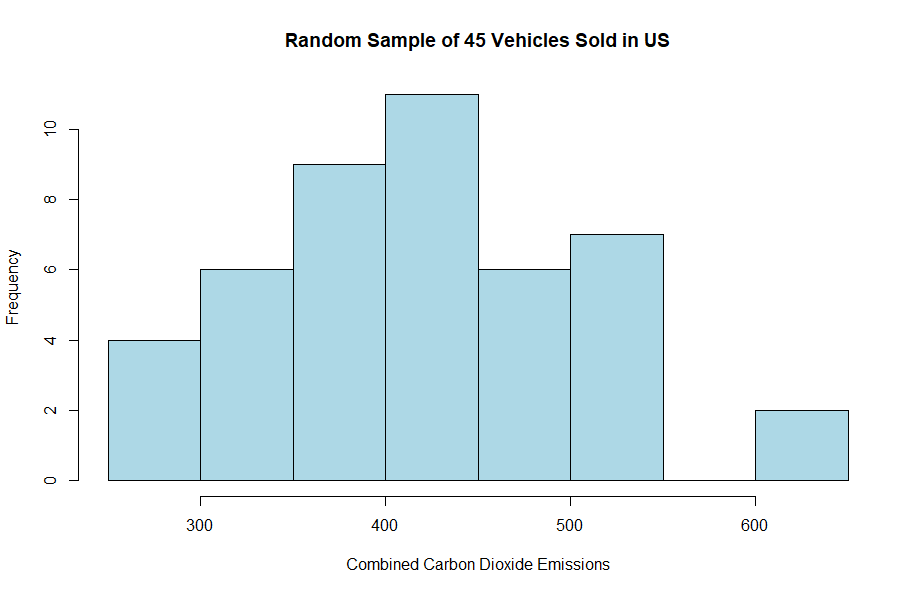
\includegraphics[width=\textwidth]{week4/Images/Rplot.png}
            
            \subsection{}
                Below I show a 95\% confidence interval given my sample from above.
                
                \[
                    Interval = X_bar +- \dfrac{z^* \sigma}{\sqrt{n}} 
                \]
                
                \[
                    = 418.267 +- \dfrac{1.96 * 89.8}{sqrt{45}} = [392.86 , 443.612]
                \]\\
                
                The interval above does contain the population mean for co2 emissions.\\
            
            \subsection{}
                I would expect that around 5\% of the students would not find the true population mean in the their 95\% confidence interval. Meaning that about 7 students answers would not contain the true population mean.\\
                
        \section{part 2}
            \subsection{}
                As mentioned above in question 1.c. only about 7 students out of the whole class are going to reject the null hypothesis. It is very likely that most of us will fail to reject the null hypothesis.\\
                
            \subsection{}
                Below is the solution to the hypothesis test:
                
                \[
                    Z_stat = \dfrac{x_bar - \mu_0}{\dfrac{\sigma}{\sqrt{n}}}
                \]
                \[
                    = \dfrac{418.2667 - 399.87}{\dfrac{89.8}{\sqrt{45}}} = 1.37
                \]
                \[
                    1 - Z(1.37) = 1 - 0.9147 = 0.08353 > 0.05
                \]
            \subsection{}
                There is not convincing evidence that the sample average does not equal the true population mean. The sample estimate of the average value for CO2 emissions is 418.267 PPM with a 95\% confidence interval of 392.86 to 445.612. We have failed to reject the null hypothesis at a significance level of 0.05 with a p-value of 0.0835.\\
                
            \subsection{}
                The same data that doesn't contain the true population mean will also reject the null hypothesis because that sample is out side of the 95\% interval and exists out side the 0.05 value we have set for Alpha.\\
                
        
        \section{part 3}
            \subsection{}
                According to the central limit theorem the distribution of the sample means will be normal. In theory the theoretically mean would be the same as the population mean at 399.87. The calculation for the standard deviation is shown below.
                
                \[
                    sd = \dfrac{\sigma}{\sqrt{n}}
                \]
                
                \[
                    = \dfrac{89.8}{\sqrt{45}} = 13.386
                \]
            \subsection{}
                The shape of the histogram appears as I would have expected normal centered around 400. The mean of the samples was 399.937 which is very close to our expected mean. The standard deviation of the samples was also close to our expected value of 13.120. This supports the central limit theorem.\\
                
                % insert image here.
                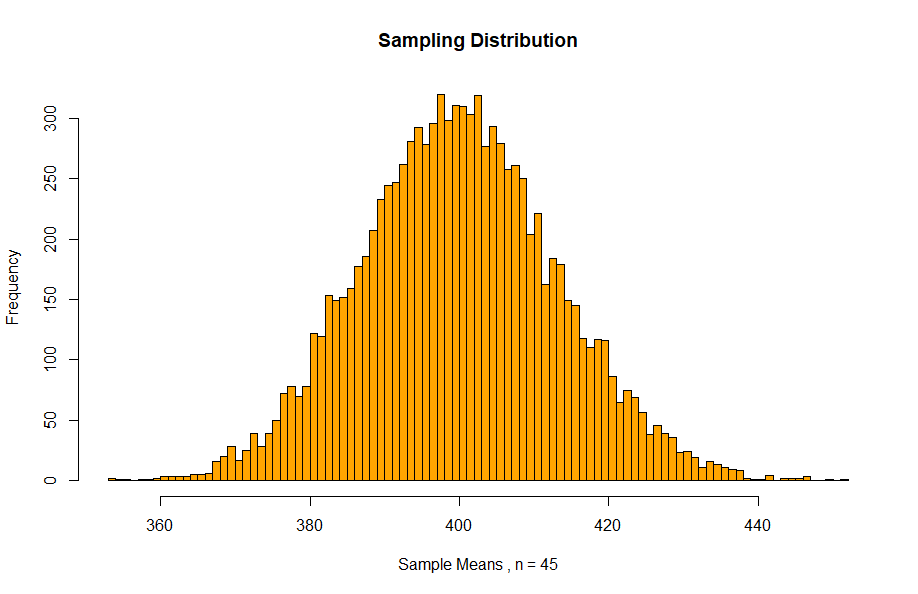
\includegraphics[width=\textwidth]{week4/Images/Rplot01.png}
                
            \subsection{}
                The Z statics can be modeled by the standard normal distribution. They should be centered around zero and have a bell shaped curve.\\
                
                % Insert Image Here.
                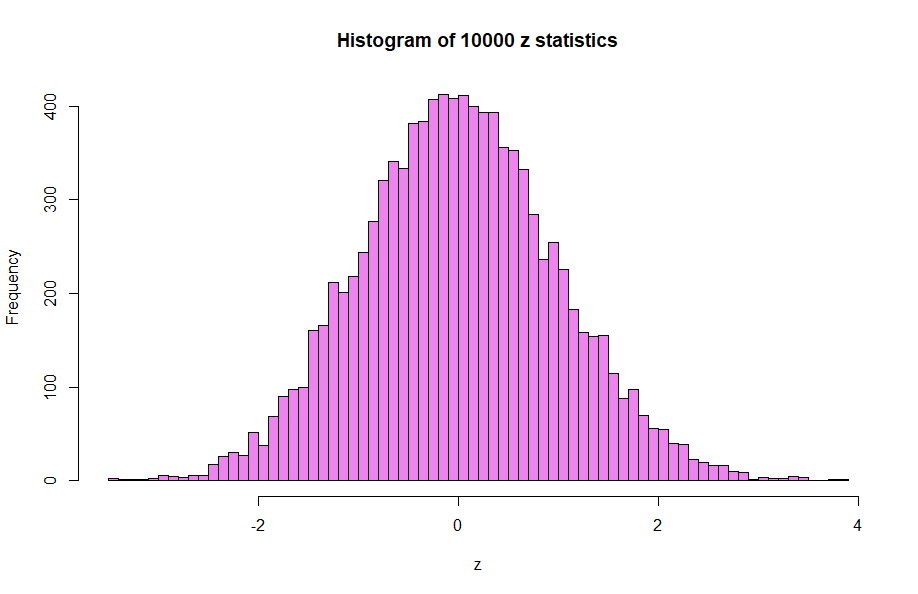
\includegraphics[width=\textwidth]{week4/Images/Rplot02.png}
                
            \subsection{}
                In this case it appears we reject the null hypothesis about 5 percent of the time. This seems to be inline with what we would expect with Alpha equal to 0.05. In the case where we reject the null hypothesis we are making a Type 1 error because we are rejecting the null hypothesis when it is true.\\
            
                % Insert plot here
                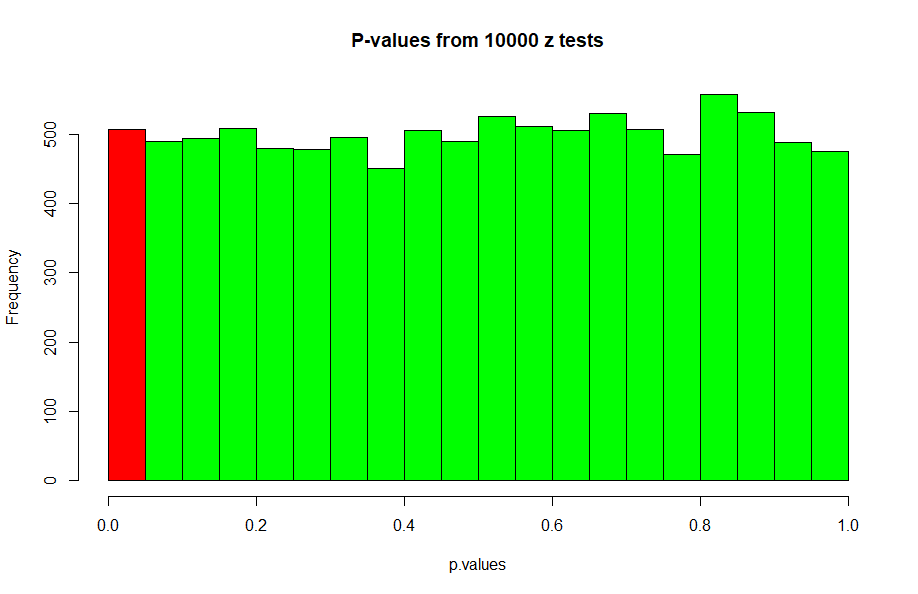
\includegraphics[width=\textwidth]{week4/Images/Rplot03.png}
        
		
		
		\section{Bibliography}
		\bibliography{References}
		\end{document}